\documentclass[twoside]{article}
\usepackage[T1]{fontenc}
\usepackage{geometry}
\geometry{verbose}
\usepackage{fancyhdr}
\pagestyle{fancy}
\setlength\parskip{\medskipamount}
\setlength\parindent{0pt}
\usepackage{graphicx}
\usepackage{fmtcount}
\usepackage{enumerate}
\usepackage{mathrsfs}

% original values
% \setlength\topmargin{0.25in}
% \addtolength{\hoffset}{-1.0cm}
% \addtolength{\textwidth}{2.0cm}
% \addtolength{\voffset}{-1.5cm}
% \addtolength{\textheight}{3.5cm}
%
% new ones.
\setlength\topmargin{0.7in}
\addtolength{\hoffset}{-1.0cm}
\addtolength{\textwidth}{2.0cm}
\addtolength{\voffset}{-1.5cm}
\addtolength{\textheight}{3.5cm}
% pdf ones.
%\setlength\topmargin{0.0in}
%\addtolength{\hoffset}{-1.0cm}
%\addtolength{\textwidth}{2.0cm}
%\addtolength{\voffset}{-1.5cm}
%\addtolength{\textheight}{3.5cm}

% introduce new commands here.
\makeatletter % changes the catcode of @ to 11

% two new commands to do labelling. - gpg 12/4/13
\newcommand{\customlabel}[2]{%
\protected@write \@auxout {}{\string \newlabel {#1}{{#2}{}}}}

\newcommand{\actlabel}[1]{%
\protected@write \@auxout {}{\string \newlabel {#1}{{\arabic{activity}}{}}}}

%% Special footnote code from the package 'stblftnt.sty' needed to put footnote
%% on section title
%% Author: Robin Fairbairns -- Last revised Dec 13 1996
\let\SF@@footnote\footnote
\def\footnote{\ifx\protect\@typeset@protect
    \expandafter\SF@@footnote
  \else
    \expandafter\SF@gobble@opt
  \fi
}
\expandafter\def\csname SF@gobble@opt \endcsname{\@ifnextchar[%]
  \SF@gobble@twobracket
  \@gobble
}
\edef\SF@gobble@opt{\noexpand\protect
  \expandafter\noexpand\csname SF@gobble@opt \endcsname}
\def\SF@gobble@twobracket[#1]#2{}

\makeatother % changes the catcode of @ back to 12
% end of new commands.

\newcounter{activity}

\begin{document}


\title{Investigative Physics\\ Activity Units for IQS Physics-S2}


\author{E.F. Bunn,$^1$ M.S. Fetea,$^1$
G.P. Gilfoyle,$^1$ H. Nebel,$^1$ S.Serej,$^1$ \\ P.D. Rubin,$^2$ and M.F. Vineyard$^3$\\[8pt]
$^1$Department of Physics, University of Richmond, VA 23173 \\[4pt]
$^2$Department of Physics, George Mason University, Fairfax, VA  22030 \\[4pt]
$^3$Department of Physics, Union College, Schenectady, NY 12308}

\maketitle
\begin{abstract}
The exercises in this manual have been developed to support an investigative
physics course that emphasizes active learning. Some of these units have been
taken from the Workshop Physics project at Dickinson College and the Tools for
Scientific Thinking project at Tufts University and modified for use at the
University of Richmond. Others have been developed locally.

The units are made up of activities designed to guide your investigations in
the laboratory. The written work will consist primarily of documenting your
class activities by filling in the entries in the spaces provided in the units.
The entries consist of observations, derivations, calculations, and answers
to questions. Although you may use the same data and graphs as your partner(s)
and discuss concepts with your classmates, all entries should reflect your own
understanding of the concepts and the meaning of the data and graphs you are
presenting. Thus, each entry should be written in your own words. Indeed, it
is very important to your success in this course that your entries reflect a
sound understanding of the phenomena you are observing and analyzing.

We wish to acknowledge the support we have received for this project from the
University of Richmond and the Instrumentation and Laboratory Improvement program 
of the National Science Foundation. Also, we would like to thank our laboratory 
directors for their invaluable technical assistance.
\end{abstract}

\begin{center}

%\includegraphics[width=3.4in]{el_nino1.ps}
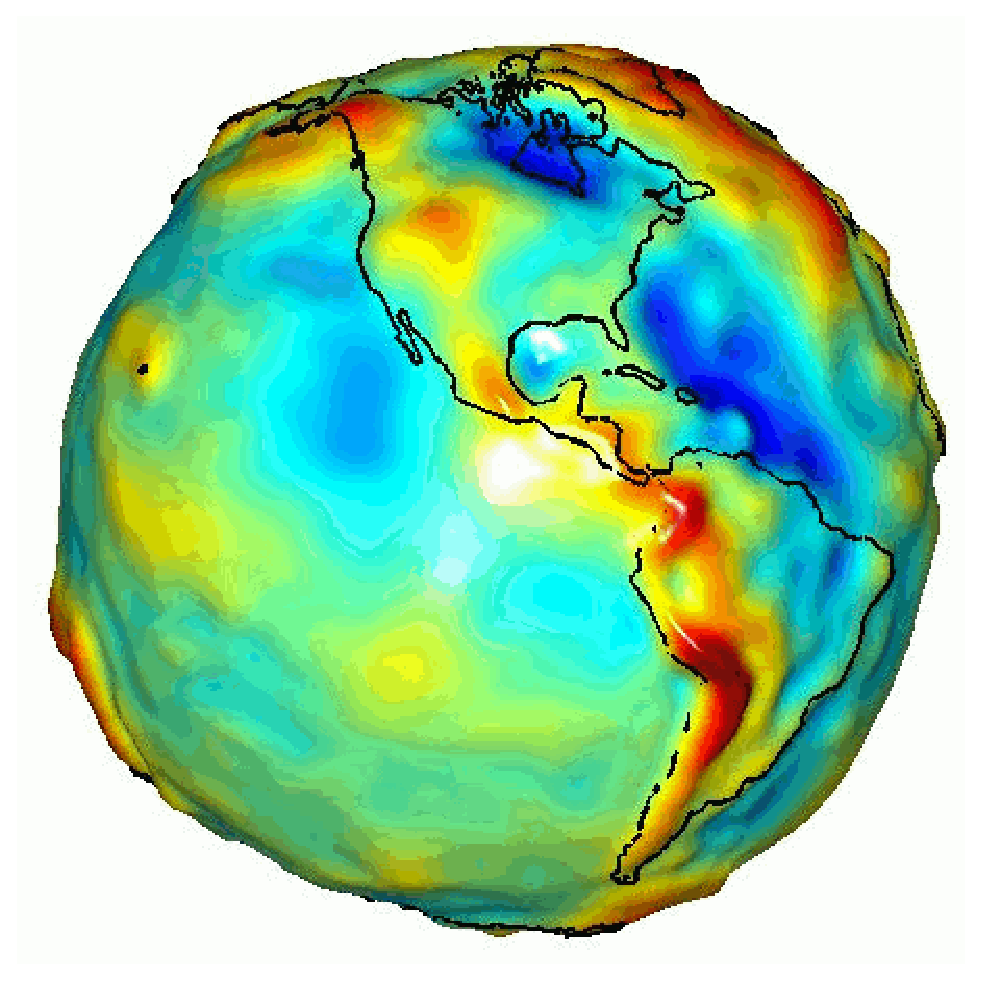
\includegraphics[width=3.4in]{grace1-1.ps}

\end{center}

\thispagestyle{empty}

\newpage


\ 
\setcounter{page}{1}

\vfill

%Cover art: Better knowledge of ocean circulation is enabling us to better understand and predict climate, 
%especially natural catastrophes such as El Ni\~ no. 
%This phenomenon, caused by anomalous warm water arrivals on the coast of Peru, 
%brings severe weather patterns, such as drought, flooding, and cyclones.

Cover art: The Gravity Recovery And Climate Experiment (GRACE) is a joint mission of NASA and the German Aerospace Center. 
It has been making detailed measurements of Earth's gravity field anomalies since its launch in March 2002.
Two spacecraft are about 140 miles apart and use microwave ranging to determine their separation to within $10~\mu m$.

\pagebreak

\tableofcontents{}

\newpage

\setcounter{page}{3}

\thispagestyle{plain}

\vfill

\ 

\pagebreak

%\setcounter{activity}{0}
%
\section{Hooke's Law}

Name \rule{2.0in}{0.1pt}\hfill{}Section \rule{1.0in}{0.1pt}\hfill{}Date \rule{1.0in}{0.1pt}

{\noindent \bf Objectives:} \begin{list}{$\bullet$}{\itemsep0pt \parsep0pt}

\item To explore the nature of elastic deformation and restoring forces

\end{list}

\noindent {\bf Introduction} 

There is no such thing as a perfectly rigid body. The stiffest of metal bars can be twisted, bent, stretched, and compressed. Delicate measurements show that even small forces cause these distortions. Under certain circumstances (typically, when the forces are not too large), a body deformed by forces acting upon it will return to its original size and shape when the forces are removed, a capacity known as elasticity. Permanent distortion from large forces is referred to as plastic deformation. In this lab, you will stay within the elastic limit. \\

{\noindent \bf Apparatus:} \begin{list}{$\bullet$}{\itemsep0pt \parsep0pt}

\item two springs and supports \item collection of masses \item 2-meter stick

\end{list}

{\noindent \bf Activity:} \begin{enumerate}

%\item  Record the mass of the two springs.

%\begin{displaymath} m_1 = \hskip50pt  m_2 = \end{displaymath}

\item  Suspend one of the springs from the support. Using the meter stick, observe the position of the lower end of the spring and record the value in the table below.

\item  Hang 100 grams from the lower end of the spring and again record the position of this end.

\item  Repeat 2 with loads of 200, 300, 400, and 500 grams hung from the spring.

\item  Repeat 2 and 3 with the second spring.

\begin{center} \begin{tabular}{||c|c|c||c|c|c||} \hline \hline Mass suspended & Position & Elongation & Mass suspended & Position & Elongation \\ from spring 1 & reading & & from spring 2 & reading & \\ (g) & (m) & (m) & (g) & (m) & (m) \\ \hline \hline 0 & & 0 & 0 & & 0 \\ \hline 100 & & & 100 & & \\ \hline 200 & & & 200 & & \\ \hline 300 & & & 300 & & \\ \hline 400 & & & 400 & & \\ \hline 500 & & & 500 & & \\ \hline \hline \end{tabular} \end{center}

\item Determine the elongation produced by each load.

\item  Plot a curve using the values of the elongation as the abscissas (x values) and the forces due to the corresponding loads as ordinates (y values) for each spring. Make sure you use compatible units. Write the equation for each curve in the space below.

\vskip70pt

\end{enumerate}

\pagebreak

\textbf{Questions:}

\begin{enumerate}
\item What do your curves show about the dependence of each spring's elongation upon the applied force?\vspace{30mm}

\item List the proportionality constant (including proper units) for each spring in the space below.\vspace{30mm}

\item The slope of each line (the proportionality constant) is known as the force constant, $k$. Which spring has the larger force constant? Express in your own words the physical implications of different size force constants.
\end{enumerate}


\setcounter{activity}{0}
\section{Periodic Motion}

Name \rule{2.0in}{0.1pt}\hfill{}Section \rule{1.0in}{0.1pt}\hfill{}Date \rule{1.0in}{0.1pt}

{\bf Objectives }

To learn directly about some of the characteristics of periodic motion, 
namely period, frequency, and amplitude from the motion of a mass hanging from a spring. 
We will also investigate the relationships between position, velocity, acceleration, 
and force in simple harmonic motion.
Last, we will test the conservation of energy in simple harmonic motion.


\textbf{Apparatus} 

\begin{tabular}{p{2.5in}p{2.5in}}
$\bullet$  Spring                         & $\bullet$  Motion detector   \\[5pt]
$\bullet$  \textit{Pasco 750 Interface}   & $\bullet$  Force probe       \\[5pt]
$\bullet$  Variety of masses              & $\bullet$  \textit{DataStudio} software \\[5pt]
$\bullet$  2-meter stick                  &  \\[5pt]
\end{tabular}

%\begin{tabular}{|l|l|l|} \hline
%Two springs & Motion detector   & \textit{Science Workshop 750 Interface} \\ \hline
%Force probe & Variety of masses & \textit{DataStudio} software (Position and Velocity Graphs, SHM) \\ \hline
%\end{tabular}

\textbf{Introduction }

Periodic motion is motion that repeats itself. You can see the repetition in
the position-, velocity-, or acceleration-time graphs. The length of time to
go through one cycle and begin to repeat the motion is called the period $T$. The
number of cycles in each second is called the frequency $f$. The unit of frequency,
cycles per second, is given a special name --- Hertz.


\textbf{Activity  \stepcounter{activity}\arabic{activity}: Determination of the Spring Constant }

Measure the distance the spring stretches for five different masses and use
these data to determine the spring constant, $k$. 
Record your data and the result for $k$ in the space below.
\vspace{50mm}



\textbf{Activity  \stepcounter{activity}\arabic{activity}: Periodic Motion of a Mass-Spring System}

(a) Open the \textbf{Position \& Velocity Graphs} application in the \textbf{131 Workshop} submenu. 
Hang the large spring from the force probe hook with the
large diameter coils down and hang a 200-g mass from the spring. 
Place the motion detector facing up directly below the spring. 
Pull the mass straight downward about $7~ cm$, and let go.
Be careful to pull straight down so the motion of the weight is vertical and does not
swing sideways. 
Also be careful so the weight does not fall off the spring and strike the motion sensor.
Adjust the height of the support so that the mass comes no closer than $15~cm$ to the detector. 
Record data for a few seconds to display
position-time and velocity-time graphs of the motion. Sketch the graphs on the  axes below.

\textbf{Comment}: Note that when an object returns to the same position, it does not
necessarily mean that a cycle is ending. It must return to the same position,
and the velocity and acceleration must also return to the same values in both
magnitude and direction for this to be the start of a new cycle.

\vspace{0.3cm}
{\par\centering 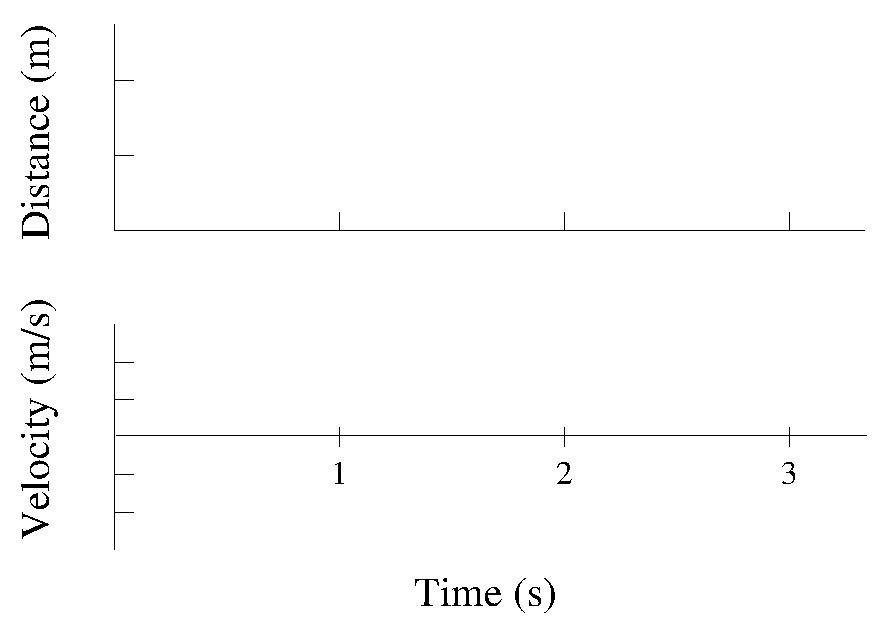
\includegraphics{periodic_motion/periodic_motion_fig1b.eps} \par}
\vspace{0.3cm}

(b) Label the graphs above with: ``B'' at the Beginning of a
cycle and ``E'' at the End of the same complete cycle, ``A''
on each spot where the mass is moving Away from the detector fastest, ``T''
on each spot where the mass is moving Toward the detector fastest, ``S''
on each spot where the mass is standing Still, ``F'' where the
mass is Farthest from the motion detector, and ``C'' where the mass
is Closest to the motion detector.

(c) Do the position and velocity graphs appear to have the same period? Do their
peaks occur at the same times? If not, how are the peaks related in time?
\vspace{20mm}

(d) Use the Smart Tool to measure the period and frequency of the motion. (For
better accuracy, measure the total time over as many cycles as possible and
divide by the number of cycles.)
\vspace{30mm}

(e) Using the Smart Tool, determine and record the maximum displacement
on your position graph. 
Next, collect data with the mass at rest hanging from the spring to find the equilibrium position. 
Subtract  this equilibrium \newpage value from the maximum displacement.
This is the amplitude of the motion.
Calculate and record here the amplitude of
the motion (the difference between the maximum displacement and the equilibrium
position).
\vspace{30mm}

\textbf{Simple Harmonic Motion }

The motion of a mass hanging from a spring that you looked at in Activity 2
is a close approximation to a kind of periodic motion called simple harmonic
motion (sometimes abbreviated SHM).

\textbf{Activity  \stepcounter{activity}\arabic{activity}: What Factors Determine the Period of the Mass-Spring System? }

(a) We now want to consider ways to change the period of the oscillator and make some predictions.
What will happen to the period if you increase the amplitude? 
\vspace{25mm}

(b) What will happen to the period if you increase the mass?
\vspace{25mm}


\textbf{Activity  \stepcounter{activity}\arabic{activity}: The Period of SHM and the Amplitude} 

(a) Repeat the procedure of Activity 2, but with a different starting position
of about 10 cm. (Warning: Do not make the amplitude so large that the mass
comes closer than 0.15 m from the motion detector.) When you have good graphs,
find and record the period and the amplitude using the methods described in
Activity 2. 
\vspace{20mm}

(b) Take ratios of the period and the amplitude of Activity 2 to those determined
here.
\vspace{20mm}

(c) Is there evidence that the period depends on amplitude? (Did the change
in amplitude result in a comparable change in period?) Explain. How does this
compare with your prediction?
\vspace{20mm}

\newpage

\textbf{Activity  \stepcounter{activity}\arabic{activity}: The Dependence of the Period of a SHM on the Mass} 

(a) Carefully measure the period for two other masses. Record the masses and
the measured periods in a table in the space below along with the mass and period from Activity 1.
\vspace{30mm}

(b) Does the period depend on the mass? Does it increase or decrease as mass
is increased?
\vspace{20mm}

\textbf{Comment:} You should have found that $T$ is independent of amplitude and increases with mass. 
The theoretical expression for the period is
\[T=2\pi \sqrt{\frac{m}{k}.}\]


\textbf{Velocity, Acceleration, Force and Energy }

In this investigation you will look more carefully at the distance, velocity
and acceleration graphs for simple harmonic motion. You will also look at the
force graph, and will examine the energy associated with simple harmonic motion.

\textbf{Activity  \stepcounter{activity}\arabic{activity}: Velocity, Acceleration, and Force for SHM} 

(a) Consider the motion you looked at in Activity 1 when the mass was 200 g
and the initial position was $5-10~ cm$. Sketch the position and velocity graphs
that you observed on the axes below using dashed lines.

\vspace{0.3cm}
{\par\centering 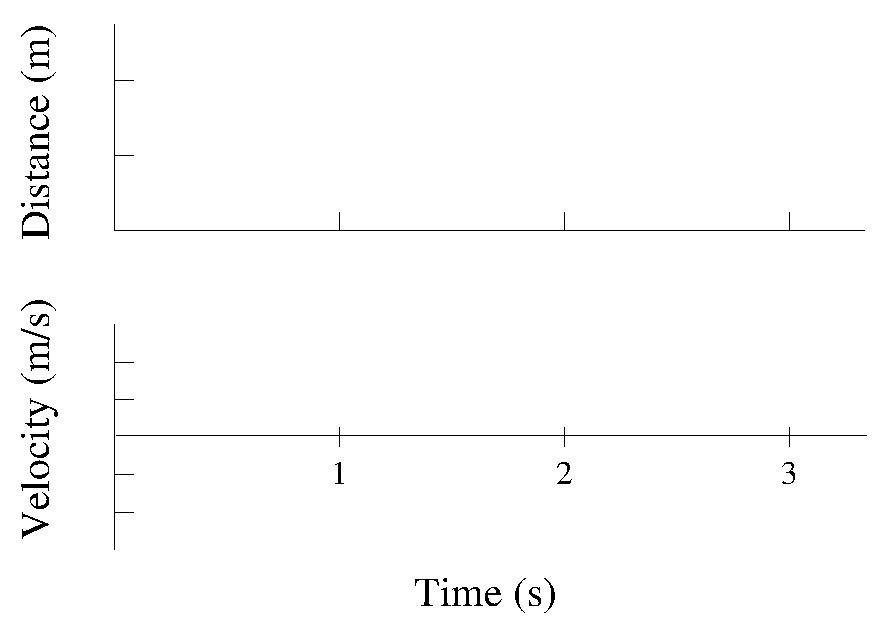
\includegraphics[width=4.0in]{periodic_motion/periodic_motion_fig1b.eps} \par}
\vspace{0.3cm}

\newpage

(b) Based on what you know about the relationships between velocity, acceleration,
and force, use dashed lines to sketch your predictions for the acceleration
and force graphs.

\vspace{0.3cm}
{\par\centering 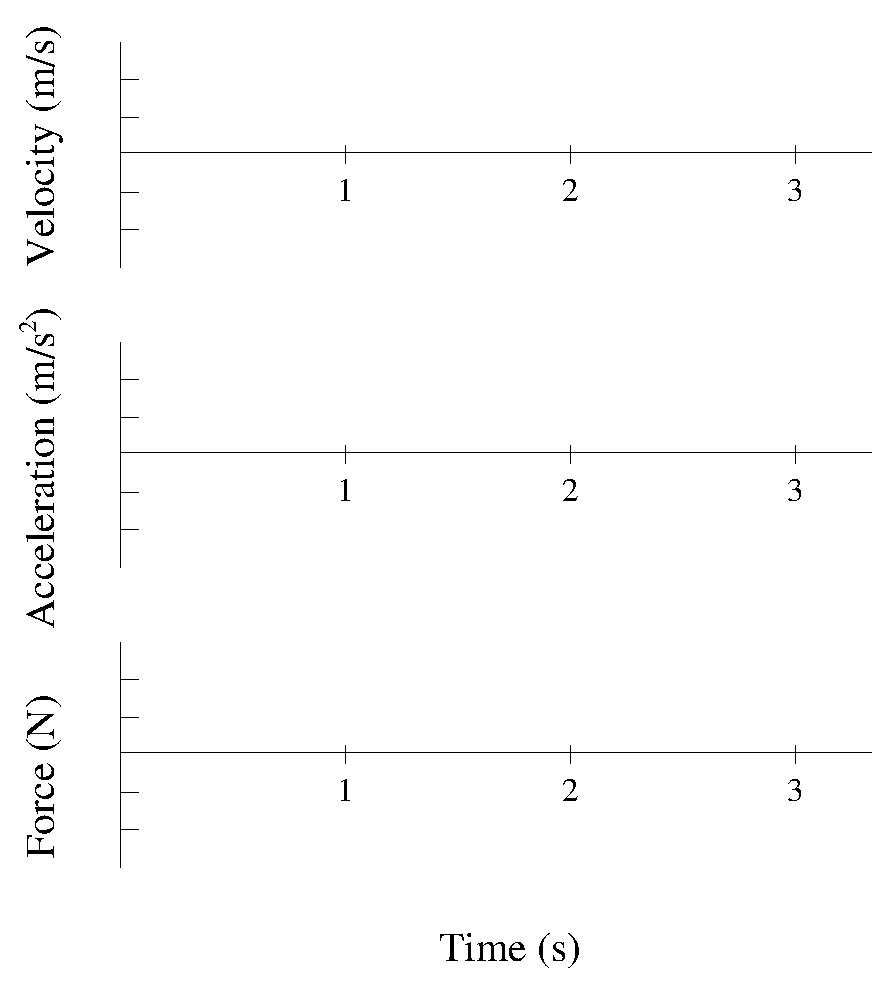
\includegraphics[width=4.0in]{periodic_motion/periodic_motion_fig3b.eps} \par}
\vspace{0.3cm}

(c) Suspend the 200-g mass from the spring and 
open the \textbf{SHM} application in the \textbf{131 Workshop} submenu. 
Start the mass oscillating with an amplitude of $5-10~ cm$ and record data for a few seconds.
When you have obtained good graphs, sketch the results on the above axes using
solid lines. Print your graph and attach to this unit.

(d) When the mass is at its maximum distance from the detector, is the velocity
maximum, minimum or some other value according to your graphs? Does this agree
with your predictions? Does this agree with your observations of the oscillating
mass? Explain.
\vspace{15mm}

(e) When the mass has its maximum positive velocity, is its distance from the
detector maximum, minimum, the equilibrium value or some other value according
to your graphs? What about when it reaches maximum negative velocity? Does this
agree with your predictions? Does this agree with your observations of the oscillating mass? Explain. 
\vspace{20mm}

\newpage

(f) According to your graphs, for what distances from the detector is the acceleration
maximum? For what distances is the acceleration zero? What is the velocity in
each of these cases?
\vspace{20mm}

(g) Compare the force and acceleration-time graphs. Describe any similarities.
Does the force graph agree with your prediction?
\vspace{20mm}

(h) From your graphs, what would you say is the relationship between force and
acceleration? 
\vspace{20mm}

(i) Compare the force and distance(position)-time graphs. What would you say
is the relationship between force and position? 
\vspace{20mm}

\textbf{Activity  \stepcounter{activity}\arabic{activity}: Energy of a Mass Undergoing SHM }

Now use the {\it DataStudio} graphs from the last activity to examine the energy relationships
in simple harmonic motion. 
To get the displacement from equilibrium you have to estimate the equilibrium position
on your position vs. time plot.
You can do this with the {\it SmartTool} by finding the point halfway between the 
minimum and maximum values of each 
oscillation.
The $x$ values must be determined relative to this equilibrium position (which represents a displacement of zero).
You will subtract this equilibrium value from the position measurement to get the displacement in
your analysis below.
Also, make sure the time axes for each graph are aligned.

(a) If we place the origin at the equilibrium point of the spring,
then where is the kinetic energy of the mass zero? Label these points
on your distance and velocity graphs above with a K.

(b) Calculate the elastic potential energy due to the spring at one of these
points. Label the point you use on your velocity and distance graphs with a
1. Use $U = {1\over 2}kx^{2}$, where 
$x$ is the distance from the equilibrium position
and $k$ is the force constant of the spring, 
which you have already measured in Activity 1. Use
the Smart Tool to measure $x$. Show your data and calculations in the space below. 
\vspace{20mm}

(c) Where is the potential energy zero? Label these points with a P
on your distance and velocity graphs.

(d) If you measured the kinetic energy at one of these points, what would you
expect its value to be? Explain.
\vspace{20mm}

\newpage

(e) Check your prediction. Calculate the kinetic energy at one of these points.
Label the point you use on your velocity graph with a 2. Use 
$K = {1\over 2} mv^{2}$.
Use the Smart Tool to determine $v$. Show your data and calculations in the space
below.
\vspace{20mm}

(f) Did your calculated kinetic energy agree with your prediction?
\vspace{20mm}

(g) If you calculated the potential and kinetic energies at a point where neither
of these was zero, what would you expect the total energy to be? Explain.
\vspace{20mm}

(h) Check your prediction. Make a table below (or make a spreadsheet and attach it to this unit)
with headings for $v~(m/s)$, position ($m$), $x~(m)$ where $x$ is the difference between the position
of the mass and the equilibrium position, $K$, $U$, and the total energy.
Pick at least six points where the mass has both kinetic and
potential energy, calculate them both ($K$ and $U$), and then calculate the total energy for each point ($K+U$). 
Label these points on your distance
and velocity graphs with numbers. 
Calculate the average and standard deviation of the total mechanical energy.
For information on calculating the average and
standard deviation, see \textbf{Appendix A}. Record the average and standard deviation here.
\vspace{60mm}

(i)  Is the total energy conserved?  Be quantitative in your answer.



\setcounter{activity}{0}
P7 332
#XVVERSION:version 3.10a-jumboFix+Enh of 20081216 (interim!)+FLmask
#BUILTIN:UNKNOWN
#IMGINFO:
#END_OF_COMMENTS


%\setcounter{activity}{0}
%
\section{Connecting Angular Displacement and Linear Displacement}

Name \rule{2.0in}{0.1pt}\hfill{}Section \rule{1.0in}{0.1pt}\hfill{}Date \rule{1.0in}{0.1pt}

{\noindent \bf Objectives:}

\begin{list}{$\bullet$}{\itemsep0pt \parsep0pt}

\item Discover the relationship between arc length, radius, and angle \item Understand radian measure

\end{list}

\textbf{Apparatus}

\begin{itemize}
\item Wooden disks
\item Meter stick
\item String
\end{itemize}
\textbf{Activity  \stepcounter{activity}\arabic{activity}: Measuring Circular Quantities} 

\begin{enumerate}

\item With the string and meter stick, determine the circumference of the disk in cm.

\bigskip

\begin{center} circumference = \rule{3cm}{0.4pt} \end{center}

\item Calculate the disk's diameter and radius.

\bigskip

\begin{center} diameter = \rule{3cm}{0.4pt} \hspace{1cm} radius = \rule{3cm}{0.4pt} \end{center}

\item Check that the meter stick is inserted in the base with the scale visible.

\item Be sure the string is attached at the 0-mark on the disk. Wind the string around the disk one full rotation so that the 0-mark and the beginning of the string are at the bottom of the disk and the string is wound around once in such a way that when you unwind it, you can pull it along the meter stick and the disk will rotate counter-clockwise.

\item In this configuration, note the position of the tag on the string with reference to the meter stick.

\item While keeping the string taut, pull it gently to displace the tag five centimeters. Record in the table below the angular position of the bottom of the disk.

\item Repeat step 6 in five centimeter increments until the string is completely unwound.

\item Calculate the angular displacements and plot linear displacement versus angular displacement.

\end{enumerate}

\pagebreak

\begin{center} \tabcolsep1cm \setlength{\unitlength}{1mm} \begin{tabular}{|c|c|c|} \hline $\Delta s$ & $\theta$ & $\Delta\theta$ \\ (cm) & (rad) & (rad) \\ \hline \hline 5.0&& \\ \hline 10.0&& \\ \hline 15.0&& \\ \hline 20.0&& \\ \hline 25.0&& \\ \hline 30.0&& \\ \hline 35.0&& \\ \hline 40.0&& \\ \hline 45.0&& \\ \hline \end{tabular} \end{center}

\smallskip

{\noindent \bf Questions:}

\begin{enumerate}
\item Do your data points appear to fall on a line? Did you expect them to? Explain. \vspace{15mm}

\item If you were to fit a line through these points, would that line go through the
origin? Explain. \vspace{15mm}

\item Fit a line through the data. Express in words the meaning of the slope. What
is its physical interpretation? \vspace{15mm}

\item If a bigger disk were used, what would your result be? For a given angular displacement
of the bigger disk, how would the linear displacement differ? \vspace{15mm}

\item What is the ratio of some arc length to the radius of the disk? \vspace{15mm}

\item The unit given for the angular displacement is rad, which is an abbreviation
for radians. Express, in words, the meaning of the term. \vspace{15mm}

\item How many radians are in half the circumference of the disk? In the whole circumference?
\end{enumerate}


\setcounter{activity}{0}

\section{Introduction to Rotation\footnote{
1990-93 Dept. of Physics and Astronomy, Dickinson College. Supported by FIPSE
(U.S. Dept. of Ed.) and NSF. Portions of this material may have been modified
locally and may not have been classroom tested at Dickinson College.
}}

Name \rule{2.0in}{0.1pt}\hfill{}Section \rule{1.0in}{0.1pt}\hfill{}Date \rule{1.0in}{0.1pt}

\textbf{Objectives} 

To understand the definitions of angular velocity and angular acceleration and
the kinematic equations for rotational motion on the basis of observations.
We will discover the relationship between linear velocity and angular velocity
and between linear acceleration and angular acceleration.

\textbf{Apparatus}

\begin{itemize}
\item A rotator consisting of an axle, a metal disk, and a fixture to hold the disk. 
\item A stopwatch. 
\item A meter stick, drawing compass, flexible ruler, protractor, and some string.
\end{itemize}
\textbf{Overview }

Earlier in the course, we studied centripetal force and acceleration, which
characterize circular motion. In general, however, we have focused on studying
motion along a straight line as well as the motion of projectiles. We have defined
several measurable quantities to help us describe linear and parabolic motion,
including position, velocity, acceleration, force, and mass. In the real world,
many objects undergo circular motion and/or rotate while they move. The electron
orbiting a proton in a hydrogen atom, an ice skater spinning, and a hammer that
tumbles about while its center of mass moves along a parabolic path are just
three of many rotating objects. 

Since many objects undergo rotational motion it is useful to be able to describe
their motions mathematically. The study of rotational motion is also very useful
in obtaining a deeper understanding of the nature of linear and parabolic motion.

We are going to try to define several new quantities and relationships to help
us describe the rotational motion of rigid objects, i.e., objects that do not
change shape. These quantities will include angular velocity, angular acceleration,
rotational inertia and torque. We will then use these new concepts to develop
an extension of Newton's second law to describe rotational motion for masses
more or less concentrated at a single point in space (e.g., the electron in
the hydrogen atom) and for extended objects (like the tumbling hammer).

\textbf{Rigid vs. Non-rigid Objects} 

We will begin our study of rotational motion with a consideration of some characteristics
of the rotation of rigid objects about a fixed axis of rotation. The motions
of objects, such as clouds, that change size and shape as time passes are hard
to analyze mathematically. In this unit we will focus primarily on the study
of the rotation of particles and rigid objects around an axis that is not moving.
A rigid object is defined as an object that can move along a line or can rotate
without the relative distances between its parts changing. 

Shown in the figure below are examples of a non-rigid object in the form of
a cloud that can change shape and of a rigid object in the form of an empty
coffee cup that does not change shape.

\vspace{0.3cm}
{\par\centering 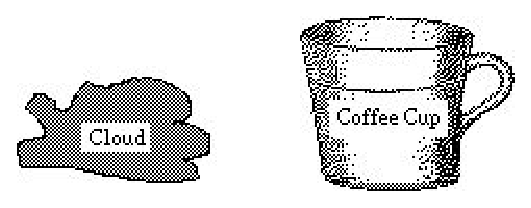
\includegraphics{rotation/rotation_fig1.eps} \par}
\vspace{0.3cm}

A hammer tossed end over end and an empty coffee cup are examples of rigid objects.
A ball of clay that deforms permanently in a collision and a cloud that grows
are examples of non-rigid objects. 
\vspace{0.3cm}

\textbf{A Puzzler} 

Use your imagination to solve the rotational puzzler outlined below. It's one
that might stump someone who hasn't taken physics.

\textbf{Activity  \stepcounter{activity}\arabic{activity}: Horses of a Different Speed }

You are on a white horse, riding off at sunset with your beau on a chestnut
mare riding at your side. Your horse has a speed of 4.0 m/s and your beau's
horse has a speed of 3.5 m/s, yet he/she constantly remains at your side. Where
are your horses? Make a sketch to explain your answer.

\vspace{0.3cm}
{\par\raggedright 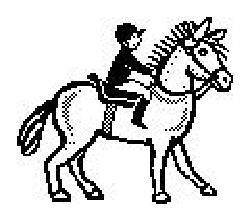
\includegraphics{rotation/rotation_fig3.eps} \par}
\vspace{0.3cm}

\textbf{Review of the Geometry of Circles }

Remember way back before you came to college when you studied equations for
the circumference and the area of a circle? Let's review those equations now,
since you'll need them a lot from here on in.

\textbf{Activity  \stepcounter{activity}\arabic{activity}: Circular Geometry} 

(a) What is the equation for the circumference, $C$, of a circle of radius $r$?
What are the units of $C$?

\vspace{0.3cm}
{\par\raggedright 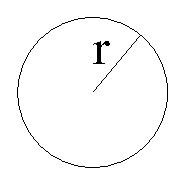
\includegraphics[height=2.0cm]{rotation/circle1.eps} \par}
\vspace{0.3cm}

(b) What is the equation for the area, $A$, of a circle of radius r? What are
the units of $A$?
\vspace{10mm}

(c) If someone told you that the area of a circle was $A = r$, how could you refute
them immediately? What's wrong with the idea of area being proportional to $r$?
\vspace{20mm}

\textbf{Distance from an Axis of Rotation and Speed }

Let's begin our study by examining the rotation of objects about a common axis
that is fixed. What happens to the speeds of different parts of a rigid object
that rotates about a common axis? How does the speed of the object depend on
its distance from an axis? You should be able to answer this question by observing
the rotational speed of the rotator at each experimental station.

\vspace{0.3cm}
{\par\centering 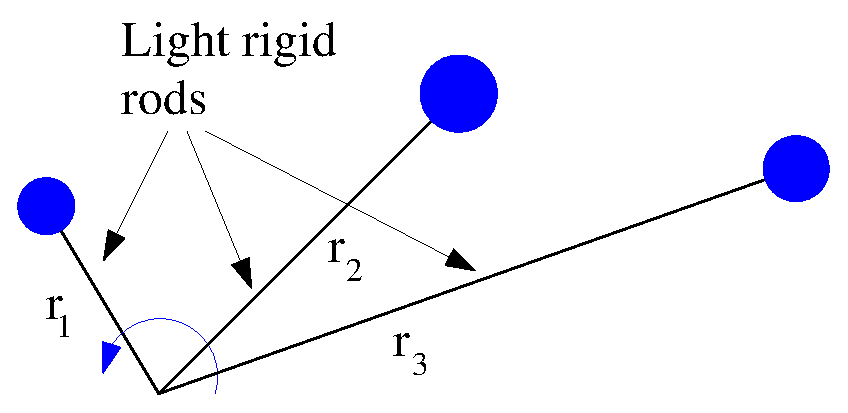
\includegraphics[height=4.0cm]{rotation/lightRods.eps} \par}
\vspace{0.3cm}

Place the disk in the fixture and slowly rotate it a constant speed. The figure
below shows the rotator and the definition of angular displacement.

\vspace{0.3cm}
{\par\centering 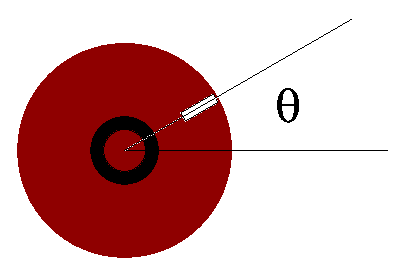
\includegraphics[height=3.0cm]{rotation/rotator.eps} \par}
\vspace{0.3cm}

\textbf{Activity  \stepcounter{activity}\arabic{activity}: Spinning the Rotator: Speed vs. Radius} 

(a) Measure how long it takes the white marker to sweep through a known angle.
Record the time and the angle in the space below.
\vspace{10mm}

(b) Calculate the distance of the paths traced out by the outer edge of the white marker 
and the inner edge as it rotated through the angle you just recorded.
(Note: What do you need to measure to perform this calculation?) Record your
data below.
\vspace{20mm}

(c) Calculate the average speed of the outer edge of the white marker and the
average speed of the inner edge of the marker. How do they compare?
\vspace{20mm}

(d) Do the speeds seem to be related in any way to the distances of inner and
outer edges of the white marker from the axis of rotation? If so, describe the
relationship mathematically.
\vspace{18mm}

\newpage

(e) As the disk rotates, does the distance from the axis of rotation to the outer 
edge of the white marker change?
\vspace{10mm}

(f) As the disk rotates, does the distance from the axis of rotation to the inner 
edge of the white marker change?
\vspace{10mm}

(g) At any given time during your rotation, is the angle between the reference
axis and the inner edge of the white marker the same as the angle between the
axis and the outer edge of the white marker, or do the angles differ?
\vspace{10mm}

(h)At any given time during the rotation, is the rate of change of the angle
between the reference axis and the inner edge of the white marker the same as
the rate of change of the angle between the axis and the outer edge, or do the
rates differ?
\vspace{10mm}

(i) What happens to the linear velocity, \textbf{v}, of the outer edge of the
marker as it rotates at a constant rate? Hint: What happens to the magnitude
of the velocity, i.e., its speed? What happens to its direction?
\vspace{20mm}

(j) Is the outer edge of the white marker accelerating? Why or why not?
\vspace{20mm}

\textbf{Radians, Radii, and Arc Lengths} 

An understanding of the relationship between angles in radians, angles in degrees, 
and arc lengths is critical in the study of rotational motion. There are two
common units used to measure angles: degrees and radians.

\begin{enumerate}
\item A degree is defined as 1/360th of a rotation in a complete circle.
\item A radian is defined as the angle for which the arc along the circle is equal 
to its radius as shown in the figure below.
\end{enumerate}
\vspace{0.3cm}
{\par\centering 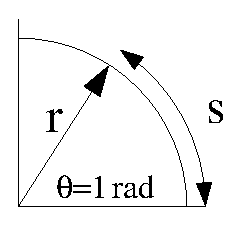
\includegraphics{rotation/radians.eps}\put(-200,40){\parbox{1.0in}{\Large $\theta =1~rad$ when $s=r$.}} \par}
\vspace{0.3cm}

In the next series of activities you will be relating angles, arc lengths, and
radii for a circle.

\textbf{Activity  \stepcounter{activity}\arabic{activity}: Relating Arcs, Radii, and Angles} 

(a) Let's warm up with a review of some very basic mathematics. What should
the constant of proportionality be between the circumference of a circle and
its radius? Write the appropriate equation.
\vspace{10mm}

(b) Approximately how many degrees are in one radian? Let's do this experimentally.
Using the compass draw a circle and measure its radius. Then, use the flexible
ruler to trace out a length of arc, s, that has the same length as the radius.
Next measure the angle in degrees that is subtended by the arc.
\vspace{50mm}

(c) Theoretically, how many degrees are in one radian? Please calculate your
result to three significant figures. Using the equation for the circumference
of a circle as a function of its radius and the constant $\pi=3.1415927$..., 
figure
out a general equation to find degrees from radians. \textbf{Hint:} How many
times does a radius fit onto the circumference of a circle? How many degrees
fit in the circumference of a circle?
\vspace{30mm}

(d) If an object moves 30 degrees on the circumference of a circle of radius
1.5 m, what is the length of its path?
\vspace{30mm}

(e) If an object moves 0.42 radians on the circumference of a circle of radius
1.5 m, what is the length of its path?
\vspace{30mm}

\newpage

(f) Remembering the relationship between the speed of the outer edge of the
rotator and the distance, $r$, 
from the rotator's axis the outer edge, what equations
would you use to define the magnitude of the average ``angular''
velocity, \( \langle\omega \rangle \)? \textbf{Hint:} In words, 
\( \langle\omega \rangle \) is defined
as the amount of angle swept out by the object per unit time. Note that the
answer is not simply \( \theta/t  \)!

\vspace{0.3cm}
{\par\raggedright 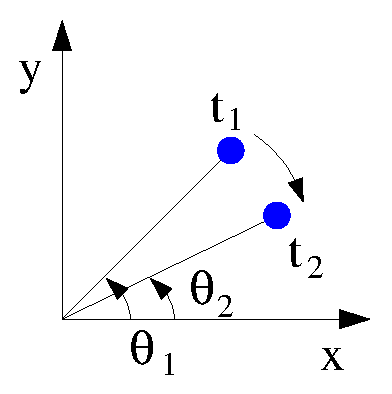
\includegraphics[height=4.5cm]{rotation/angularVelocity.eps} \par}
\vspace{0.2cm}

(g) How many radians are there in a full circle consisting of 360 degrees?
\vspace{15mm}

(h) When an object moves in a complete circle in a fixed amount of time, what
quantity (other than time) remains unchanged for circles of several different
radii? 
\vspace{15mm}

\textbf{Relating Linear and Angular Quantities} 

It's very useful to know the relationship between the variables 
$s$, $v$, and $a$,
which describe linear motion and the corresponding variables \( \theta  \),
\( \omega  \), and \( \alpha  \), which describe rotational motion. You now
know enough to define these relationships.

\textbf{Activity  \stepcounter{activity}\arabic{activity}: Linear and Angular Variables }

(a) Using the definition of the radian, what is the general relationship between
a length of arc, $s$, on a circle and the variables 
$r$ and \( \theta  \) in radians. 
\vspace{10mm}

(b) Assume that an object is moving in a circle of constant radius, $r$. 
Using the relationship you found in part (a) above, 
take the derivative of s with respect to time to find the velocity of the object. 
Show that the magnitude of the linear velocity, $v$, is related to the magnitude of the angular velocity,
\( \omega  \), by the equation \(v =  \omega r \).
\vspace{15mm}

(c) Assume that an object is accelerating in a circle of constant radius, $r$.
Using the relationship you found in part (b) above, 
take the derivative of $v$ with respect to time to find the tangential acceleration of the object. 
Show that the linear acceleration, \( a_{t} \), 
tangent to the circle is related to the angular acceleration, \( \alpha  \), 
by the equation \( a_{t}  =  \alpha  r\).
\vspace{20mm}



\setcounter{activity}{0}

\section{Newton's Second Law for Rotation\footnote{
1990-93 Dept. of Physics and Astronomy, Dickinson College. Supported by FIPSE
(U.S. Dept. of Ed.) and NSF. Portions of this material may have been modified
locally and may not have been classroom tested at Dickinson College.
}}

Name \rule{2.0in}{0.1pt}\hfill{}Section \rule{1.0in}{0.1pt}\hfill{}Date \rule{1.0in}{0.1pt}

\textbf{Objectives} 

To understand torque and its relation to angular acceleration and moment of
inertia on the basis of both observations and theory. 

\textbf{Apparatus}

\begin{itemize}
\item A Rotating Disk System 
\item A hanging mass of 200 g (for applying torque) 
\item String and pulley
\item Meter stick and ruler
\item Vernier caliper
\item Small water bubble level
\item A video analysis system.
\end{itemize}
\textbf{Overview} 

We have used the definition of moment of inertia, $I$, to determine a theoretical equation for the 
moment of inertia of a uniform disk. This equation was given by
\[
I=\frac{1}{2}Mr^{2}.\]


Does this equation adequately describe the moment of inertia of a rotating
disk system? If so, then we should find that, if we apply a known torque, \( \tau  \), 
to the disk system, its resulting angular acceleration, \( \alpha  \), is actually 
related to the system's moment of inertia, $I$, by the equation
\[
\tau =I\alpha \quad \mbox{or}\quad \alpha =\tau /I\]


The purpose of this experiment is to determine if, within the limits of experimental
uncertainty, the measured angular acceleration of a rotating disk system is
the same as its theoretical value. The theoretical value of angular acceleration 
can be calculated using theoretically determined values for the torque on the
system and its moment of inertia.

\textbf{Theoretical Calculations} 

You'll need to take some basic measurements on the rotating disk system
to determine theoretical values for $I$ and \( \tau  \). Values of moment of
inertia calculated from the dimensions of a rotating object are theoretical
because they purport to describe the resistance of an object to rotation. An
experimental value is obtained by applying a known torque to the object and
measuring the resultant angular acceleration.

\newpage

\textbf{Activity  \stepcounter{activity}\arabic{activity}: Theoretical Calculations }

(a) Calculate the theoretical value of the moment of inertia of the metal disk
using basic measurements of its radius and mass. Ignore the small hole in the
middle in your calculation (i.e. assume the disk is uniform). Be sure to state units!
\vspace{5mm}

\( r_{d} =\) \hfill{}\( M_{d}= \) \hfill{}
\vspace{5mm}

\( I_{d}= \) 
\vspace{5mm}

(b)The rotating fixture that holds the disk has a complex shape. We have determined
its moment of inertia without the disk and recorded the result on the fixture.
Record that value here. Be sure to state units.
\vspace{5mm}

\( I_{f} =\) 
\vspace{5mm}

(c) Calculate the theoretical value of the moment of inertia, $I$, of the whole
system. Don't forget to include the units.
\vspace{5mm}

$I = I_{d} + I_{f} =$
\vspace{5mm}

(d) In preparation for calculating the torque on your system, summarize the
measurements for the falling mass, $m$, and the radius of the spool that has the 
string wrapped around it in the space below. The diameter of the spool can be 
measured using the vernier caliper. Don't forget the units!
\vspace{5mm}

$m = $\hfill{}\(r_{s}= \)\hfill{} 
\vspace{5mm}

(e) Calculate the theoretical value for the torque on the rotating system as
a function of the magnitude of the hanging mass and the radius, \( r_{s} \),
of the spool, assuming the tension in the string is equal to the weight of the 
falling mass (this introduces an error of less than 1 percent).  Be sure to include units.
\vspace{5mm}

\( \tau _{th}= \)
\vspace{5mm}

(f) Based on the values of torque and moment of inertia of the system, what
is the theoretical value of the angular acceleration of the disk? What are the
units? 
\vspace{5mm}

\( \alpha _{th}= \)
\vspace{5mm}

\textbf{Activity  \stepcounter{activity}\arabic{activity}: Experimental Measurement of Angular Acceleration} 

(a) Place the video camera about 1 m above the rotator, and center the rotator in the field of view of the camera.  See
the Appendix for details.
Use the small level to ensure that the surface of the rotator is level. Place a ruler of 
known length in the field of view of the camera and parallel to one side of the frame.

(b) Place the rotator so the string will pass smoothly over the pulley and put
200 g of mass on the end of the string. Release the rotator and use the
video camera to record the motion of the disk for at least two full turns. See
the Appendix for details.

(c) Determine the angular displacement of the rotator as a function of time. 
To do this task follow the instructions in the Appendix for recording, calibrating, and analyzing a movie data file. 
\textbf{Important:} Be careful to place the origin of your coordinate system on the axle of the
rotator so the angular displacement you measure will be the desired one. 
Use a marker at or near the edge of the disk to record position for each frame. 
The resulting file should contain three columns with the values of time, x-position, and y-position for two complete revolutions.

(d) What is the expression for the angular displacement of the disk (relative to the x axis) 
in terms of the x and y positions of the marker that you recorded above? (Note that these 
positions will be relative to an origin that you placed on the axle of the rotator in part (c).)
\vspace{5mm}

\( \theta  \)= 
\vspace{5mm}

(e) We want to graph the angular displacement of the disk as a function of time.
To do this:

\begin{enumerate}
\item Export your data to an \textit{Excel} file and launch 
\textit{Excel}.

\item Calculate the angular displacement \( \theta  \) in radians for the first row
in the spreadsheet. Record the result here.
You will use this result later to check the calculations you make with 
\textit{Excel}.


$\theta =$

\item Calculating the angular position for all the data as we just did
would be horribly tedious. Instead, use an {\it Excel} formula to
figure out the angular positions.  (See Appendix C for details.)
You may find it helpful to know that there is an {\it Excel} function
ATAN2 that takes the inverse tangent of the ratio of two numbers.
For instance, if you put ``=ATAN2(C3,D3)'' into a cell, {\it Excel}
will calculate the inverse tangent of the ratio of the number
in cell D3 to the number in cell C3.  (Note that the ratio
that is taken has the second argument on top: in this case, it's 
D3/C3, not C3/D3.)

\item Does the value of the first row agree with the calculation you made in part
(2) above? If it does not check both calculations again. If that fails consult
your instructor. 
\item Graph the angular displacement (column 4) as a function of time (column 1).
You will see discontinuous jumps in your data because the function you used
in part (3) always calculates angles in the range \( -\pi  \) to \( +\pi  \).
\textbf{You must add different increments of \( 2\pi  \), \(4 \pi  \), etc. to adjust
the scale of the angular displacement.} If you don't do this step, you will not be able to do part (f) below.  You should create another
column of data in your data table containing the angular positions with
appropriate multiples of $2\pi$ added to them.
\end{enumerate}
(f) We now want to extract the angular acceleration from the data.

\begin{enumerate}
\item To describe the time dependence of the angular displacement what type of function should we use to fit the data? How are the coefficients of the polynomial related to the angular acceleration?\vspace{20mm}

\item Fit the data with a polynomial and write the resulting equation for the time
dependence of the angular position in the space below. Be sure to include the
proper units with the coefficients. (Refer to Activity 6 part (d) of the previous experiment.) Determine the experimental value for the
angular acceleration from the fit and record it below. Also, print a copy of
your plot with the fitted curve and the equation and put it in your notebook.\vspace{20mm}

\end{enumerate}

\newpage


\textbf{Activity  \stepcounter{activity}\arabic{activity}: Comparing Theory with Experiment }

(a) Summarize the theoretical and experimental values of angular acceleration. Be sure to include the proper units. Calculate the percent difference using $\Delta\alpha/\alpha_{exp}$.
\vspace{10mm}

\( \alpha _{th}= \)
\vspace{10mm}

\( \alpha _{exp}= \) 
\vspace{15mm}

(b) Record the results for $\Delta\alpha/\alpha_{exp}$ for the whole class. What is the average and standard deviation for the class's data?
Do your results confirm the theory? Be quantitative in your answer.



%\setcounter{activity}{0}
%
\section{Moment of Inertia}

Name \rule{2.0in}{0.1pt}\hfill{}Section \rule{1.0in}{0.1pt}\hfill{}Date \rule{1.0in}{0.1pt}

\textbf{Objective} 

To investigate Newton's second law of motion for rotating bodies by applying
it to determine the moment of inertia of a disk.

\textbf{Moment of Inertia} 

In this experiment you will determine the moment of inertia of a body by applying
Newton's second law of motion for rotating bodies. The moment of inertia of
a body is a measure of the tendency of the body to resist a change in its state
of rotational motion. When a net external torque, 
$\tau$, acts on a rigid body free
to rotate about some axis, an angular acceleration, 
$\alpha$, is produced that is
proportional to the torque. The proportionality constant is the moment of inertia,
$I$, of the body. This is the rotational analog of Newton's second law of motion. 

The experimental setup is shown in the figure below. The apparatus consists
of a mass, $m$, connected by a string passing over two pulleys to the drum of
a rotator.

\vspace{0.3cm}
{\par\centering 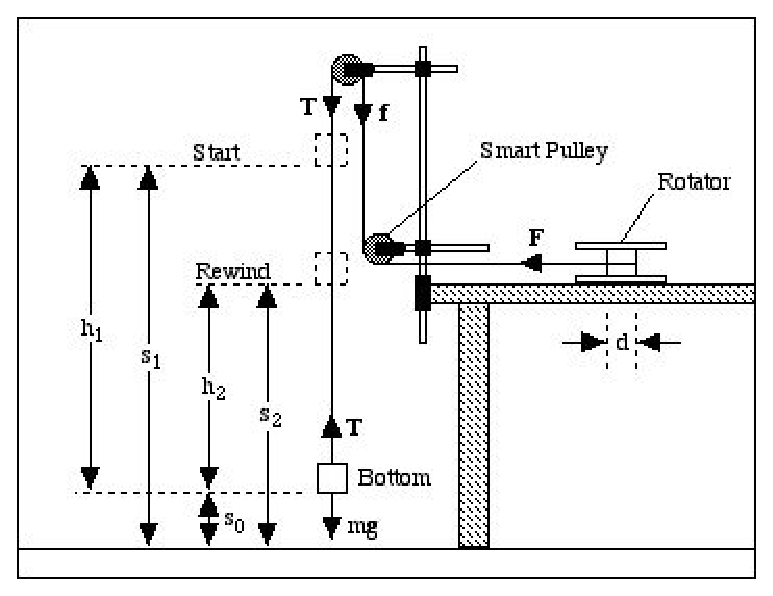
\includegraphics{moment_inertia/moment_inertia_fig1.eps} \par}
\vspace{0.3cm}

\textbf{Apparatus}

\begin{itemize}
\item Rotator
\item Smart pulley
\item Regular pulley
\item Variety of masses
\item String
\item Vernier caliper
\item 2-meter stick
\item \textit{Science Workshop 750 Interface}
\item \textit{DataStudio} software (Atwood's Machine application)
\end{itemize}
\textbf{Activity  \stepcounter{activity}\arabic{activity}: Prediction for the Moment of Inertia} 

(a) Write the symbolic expression for Newton's second law for rotating bodies
in the space below.
\vspace{10mm}

(b) Write an expression for the net torque on the rotator in terms of the radius
of the rotator drum, $r$, and the magnitude of the net force supplied by the string,
$F$.
\vspace{10mm}

(c) Write an expression for the angular acceleration of the rotator drum in
terms of the radius of the drum, $r$, and the acceleration of the hanging mass,
$a$.
\vspace{10mm}

(d) Notice that the net force on the drum, $F$, is equal to the tension in the
string, $T$, minus the frictional force, $f$. Write an expression for 
$F$ in terms
of $T$ and $f$.
\vspace{10mm}

(e) Apply Newton's second law to the hanging mass to obtain an expression for
the tension, $T$, in terms of $m$, $g$, and $a$.
\vspace{20mm}

(f) The frictional force, $f$, can be determined by application of the principle
of conservation of energy. If the mass, $m$, falls a height, \( h_{1} \), and
then rises a height, \( h_{2} \), on the rewind, the loss in its potential
energy between the two positions is equal to the work done by the frictional
force. Using this, find an expression for $f$ in terms of $m$, $g$, \( h_{1} \),
and \( h_{2} \).
\vspace{20mm}

(g) Combine the equations above, to get the following expression for the moment
of inertia of the rotator (with or without the disk): 
\[
I=\frac{md^{2}}{4a}\left( g-a-g\frac{h_{1}-h_{2}}{h_{1}+h_{2}}\right) \]
where $d$ is the diameter of the drum of the rotator.
\vspace{40mm}

\textbf{Activity  \stepcounter{activity}\arabic{activity}: Determining the Moment of Inertia }

(a) Use the vernier caliper to measure the diameter of the drum of the rotator.
Each member of the group should make an independent measurement and record the
average value as $d$. If you have questions about how to read the vernier, consult
your instructor.
\vspace{10mm}

(b) Launch the Atwood's Machine application.

(c) Remove the disk from the rotator and construct a data table below with the
column headings $m$, \( s_{0} \), \( s_{1} \), \( s_{2} \), \( h_{1} \), 
\( h_{2} \),
$a$, and $I$. Don't forget to include appropriate units in the column headings.
\vspace{100mm}

(d) Hang 50 grams on the string and lower the mass slowly until all the string
is unwound from the drum. Measure and record the distance from the bottom of
the mass to the floor as \( s_{0} \).

(e) Rewind the string on the drum until the mass is a few centimeters from the
upper pulley. Measure and record the distance, \( s_{1} \), from the floor
to the mass.

(f) Release the mass, start recording data, and stop it at its highest position
on the rewind. Measure and record the distance, \( s_{2} \), from the floor
to this position of the mass.

(g) The computer will display a graph of the velocity versus time for the fall
of the mass. Fit the data to determine the acceleration and record this value
in your data table.

(h) Repeat steps (d)-(g) two more times for a total of three trials.

(i) Replace the 50 gram mass with a 70 gram mass and repeat steps (d)-(h).

(j) Place the disk on the rotator, construct a new data table, and repeat steps
(d)-(i).
\vspace{100mm}

(k) Calculate and record the moment of inertia for each trial. Show a sample
calculation for one trial in the space below.
\vspace{30mm}

(l) Determine the average value for the moment of inertia of the rotator without
the disk and record his value as \( I_{R} \) below.
\vspace{10mm}

(m) Determine the average value for the moment of inertia of the rotator with
the disk and record this value as \( I_{R+D} \).
\vspace{10mm}

(n) Calculate and record the experimental value for the moment of inertia of
the disk, \( I_{exp}  = I_{R+D} - I_{R} \).
\vspace{10mm}

(o) Calculate the theoretical moment of inertia of the disk, \( I_{th} \),
assuming that it is uniform, and determine the \% difference between \( I_{exp} \)
and \( I_{th} \).
\vspace{40mm}

(p) Does the experimental value for the moment of inertia of the disk agree
with the theoretical value within experimental uncertainties? Do the results
verify Newton's second law of motion for rotating bodies?



%\setcounter{activity}{0}
%%% For boldface greek letters:
\def\bmath#1{\mbox{\boldmath$#1$}} 


\section{Angular Momentum and Torque as Vectors\footnote{
1990-93 Dept. of Physics and Astronomy, Dickinson College. Supported by FIPSE
(U.S. Dept. of Ed.) and NSF. Portions of this material may have been modified
locally and may not have been classroom tested at Dickinson College.
}}

Name \rule{2.0in}{0.1pt}\hfill{}Section \rule{1.0in}{0.1pt}\hfill{}Date \rule{1.0in}{0.1pt}

Objectives 

To understand the definitions of torque and angular momentum as vector quantities
and to understand the mathematical properties and some applications of the vector
cross product. We will also learn the relationship between torque and angular
momentum.

\textbf{Apparatus}

\begin{itemize}
\item A horizontal pivot
\item Vertical rod for horizontal pivot (mounted on table edge)
\item Spring scale (5 newton)
\item A ruler 
\item A protractor 
\item Rods and connectors (Styrofoam ball and bamboo skewers)
\item Two small masses (100g \& 200g) 
\item A Rotating Disk System 
\item String and pulley (with mounting clamp)
\end{itemize}
\textbf{Overview} 

This unit presents us with a consolidation and extension of the concepts in
rotational motion that you have studied so far. You studied the analogy and
relationships between rotational and linear quantities (i.e., position and angle,
linear velocity and angular velocity, linear acceleration and angular acceleration,
and force and torque) without taking into account, in any formal way, the fact
that these quantities actually behave like the mathematical entities we call
vectors. We will discuss the vector nature of rotational quantities and, in
addition, define a new vector quantity called angular momentum that is the rotational
analog of linear momentum. 

Angular momentum and torque are special vectors because they are the product
of two other vectors a position vector and a force or linear momentum vector.
To describe them we need to introduce a new type of vector product known as
the vector cross product. We will explore the definition and unique nature of
the vector cross product used to define torque and angular momentum. We will
study the relationship between torque and angular momentum as well as the theoretical
basis of the Law of Conservation of Angular Momentum.

\textbf{Observation of Torque when \( {\bf F} \) and \( {\bf r} \)
are not Perpendicular} 

Recently, you ``discovered'' that if we define torque as the
product of a lever arm and perpendicular force, an object does not rotate when
the sum of the torques acting on it add up to zero. However, we didn't consider
cases where \textbf{\( {\bf F} \)} and \textbf{\( {\bf r} \)}
are not perpendicular, and we didn't figure out a way to tell the direction
of the rotation resulting from a torque. Let's consider these complications
by generating torques as described below.

\textbf{Activity  \stepcounter{activity}\arabic{activity}: Torque as a Function of Angle} 

(a) Suppose you were to hold one of the forces in the following figure (which is a TOP view of the horizontal pivot) at an angle of 90\( ^{\circ } \)
with respect to the lever arm, \( r_{h} \), and pull on it with a steady force.
This can be done by attaching a string to the left side of the horizontal pivot, placing the string over a mounted pulley, and hanging a 200g mass on the string. Meanwhile you can attach a scale to the other end of the pivot and pull on it at several angles other than 90\( ^{\circ } \)
from its lever arm, \( r_{app} \), as shown in the figure. Would the magnitude of the balancing force be less than, greater than, or equal to the force needed at 90\( ^{\circ } \)? What do you predict? Explain. (Remember, this figure is a TOP view. Both forces in the figure should be HORIZONTAL.)

\vspace{0.3cm}
{\par\raggedright 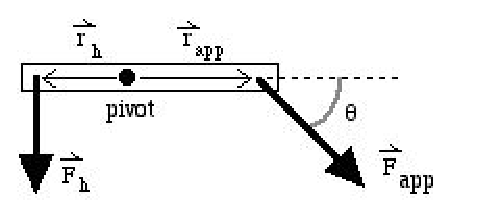
\includegraphics{ang_mom/ang_mom_fig1.eps} \par}
\vspace{0.3cm}

(b) You should determine exactly how the forces compare to that needed at a
90\( ^{\circ } \) angle. Determine this force for at least four different angles
and figure out a mathematical relationship between $F$, $r$, and \( \theta  \).
Set up a spreadsheet to do the calculations shown in the table below. Hint:
Should you multiply the product of the measured values of $r$ and $F$ 
by sin \( \theta  \)
or by cos \( \theta  \) to get a torque that is equal in magnitude to the holding
torque?

\vspace{0.3cm}
{\centering \begin{tabular}{|c|c|c|c|c|c|c|c|c|c|}
\hline 
\( r_{h} \)&
\( F_{h} \)&
\( \tau _{h} \)&
\( r_{app} \)&
\( F_{app} \)&
\( \theta  \)&
\( \cos \theta  \)&
\( \sin \theta  \)&
\( r_{app} F_{app}\cos \theta  \) &
\(r_{app} F_{app}\sin \theta  \)\\
(m)&
(N)&
(N m)&
(m)&
(N)&
(deg)&
&
&
(N m)&
(N m)\\
\hline 
\hline 
&
&
&
&
&
&
&
&
&
\\
&
&
&
&
&
&
&
&
&
\\
\hline 
&
&
&
&
&
&
&
&
&
\\
&
&
&
&
&
&
&
&
&
\\
\hline 
&
&
&
&
&
&
&
&
&
\\
&
&
&
&
&
&
&
&
&
\\
\hline 
&
&
&
&
&
&
&
&
&
\\
&
&
&
&
&
&
&
&
&
\\
\hline 
&
&
&
&
&
&
&
&
&
\\
&
&
&
&
&
&
&
&
&
\\
\hline 
\end{tabular}\par}
\vspace{0.3cm}

(c) Within the limits of uncertainty, what is the most plausible mathematical
relationship between \( \tau  \) and $r$, $F$, and \( \theta  \)?
\vspace{20mm}

The activity you just completed should give you a sense of what happens to the
magnitude of the torque when the pulling force, \( {\bf F} \), is
not perpendicular to the vector, \( {\bf r} \), from the axis of
rotation. But how do we define the direction of the rotation that results when
the torque is applied to an object that is initially at rest and not balanced
by another torque? Let's consider the directions we might associate with angular
velocity and torque in this situation.

\textbf{Activity  \stepcounter{activity}\arabic{activity}: Angular Rotation, Torque, and Direction }

(a) Suppose a particle is moving around in a circle with an angular velocity
that has a magnitude of \( \omega  \) associated with it. According to observer
\#1, does the particle appear to be moving clockwise or counter clockwise? How
about the direction of the particle's motion according to observer \#2?

\vspace{0.3cm}
{\par\raggedright 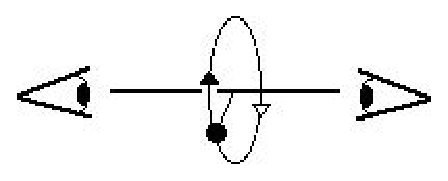
\includegraphics{ang_mom/ang_mom_fig2.eps} \par}
\vspace{0.3cm}

(b) Is the clockwise vs. counterclockwise designation a good way to determine
the direction associated with $\omega$ in an unambiguous way? Why or why not? 
\vspace{20mm}

(c) Can you devise a better way to assign a direction to an angular
velocity?
\vspace{20mm}

(d) Similar consideration needs to be given to torque as a vector. Can you devise
a rule to assign a direction to a torque? Describe the rule.
\vspace{20mm}

\textbf{Discussion of the Vector Cross Product }

An alternative to describing positive and negative changes in angle is to associate
a directed vector with the axis of rotation using an arbitrary but
well accepted rule called the right-hand rule. By using vectors we can describe
separate rotations of many body systems all rotating in different planes about
different axes. 

By using this vector assignment for direction, angular momentum and torque can
be described mathematically as ``vector cross products.'' The
vector cross product is a very strange type of vector multiplication worked
out many years ago by mathematicians who had never even heard of angular momentum or torque. The peculiar properties of the vector cross product and its relationship to angular momentum and torque are explained in most introductory physics textbooks.
The key properties of the vector that is the cross product of two vectors \( 
{\bf r} \)
and \( {\bf F} \) are that:

\begin{enumerate}
\item The magnitude of the cross product is $rF\sin\theta$ where \( \theta  \)
is the angle between the two vectors; 
\[
\left| {\bf r}\times {\bf F}\right| =\left| {\bf r}\right| \left| {\bf F}\right| \sin \theta .\]
The term \( \sin \theta  \) picks out the component of \( {\bf F} \)
along a line perpendicular to \( {\bf r} \).
\item The cross product of two vectors \( {\bf r} \) and \( {\bf F} \)
is a vector that lies in a direction perpendicular to both \( {\bf r} \)
and \( {\bf F} \) and is up if \( {\bf F} \) causes
a counter-clockwise rotation, and is down if \( {\bf F} \) causes
a clockwise rotation. These properties of the cross product are pictured below.
\end{enumerate}
\vspace{0.3cm}
{\par\centering 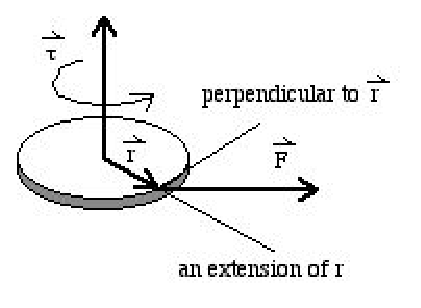
\includegraphics{ang_mom/ang_mom_fig3.eps} \par}
\vspace{0.3cm}

The spatial relationships between \( {\bf r} \), \( {\bf F} \),
and \( {\bmath{\tau} } \) are very difficult to visualize. In the next
activity you can connect some thin rods of various sizes to each other at angles
of your own choosing and make some ``vector cross products.''

\textbf{Activity  \stepcounter{activity}\arabic{activity}: Making Models of Vector Cross Products} 

(a) Pick out rods of two different lengths and connect them at some angle you
choose. Consider one of the rods to be the \( {\bf r} \) vector
and the other to be the \( {\bf F} \) vector. Measure the angle
\( \theta  \) and the lengths of \( {\bf r} \) and \( {\bf F} \)
in meters. Then compute the magnitude of the cross product as 
$rF\sin \theta $
in newton meters (N m). Show your units! Note: You should assume that the magnitude
of the force in newtons is represented by the length of the rod in meters.
\vspace{20mm}

(b) Attach a ``cross product'' rod perpendicular to the plane
determined by \( {\bf r} \) and \( {\bf F} \) with a
length of $rF\sin \theta$. Sketch the location of \( {\bf F} \)
relative to \( {\bf r} \) in the space below. Show the direction
and magnitude of the resultant torque \( {\bmath{\tau} } \). \textit{Finally,
show your cross product model to an instructor or fellow student for confirmation
of its validity. }

\vspace{0.3cm}
{\par\centering 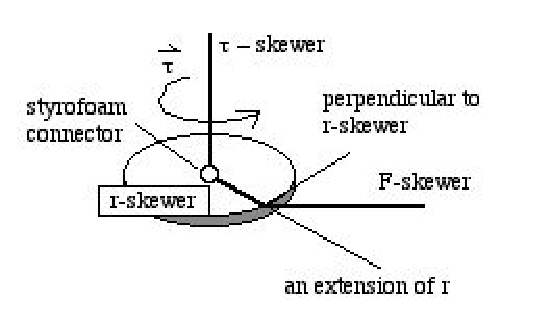
\includegraphics{ang_mom/ang_mom_fig4.eps} \par}
\vspace{0.3cm}

\textbf{Figure 2: A Model of the Vector Cross Product}

(c) In the diagrams below the vectors \( {\bf r} \) and \( {\bf F} \)
lie in the plane of the paper. Calculate the torques for the following two sets
of \( {\bf r} \) and \( {\bf F} \) vectors. In each
case measure the length of the \( {\bf r} \) vector in meters and
assume that the length of the \( {\bf F} \) vector in cm represents
the force in newtons. Use a protractor to measure the angle, \( \theta  \),
between the extension of the \( {\bf r} \)-vector and the \( {\bf F} \)-vector.
Calculate the magnitude of the torques. Place the appropriate symbol to indicate
the direction of the torque in the circle as follows: a circle with an x in
it indicates a vector into the page, while a circle with a dot in it indicates
a vector out of the page.

\vspace{0.3cm}
{\par\centering 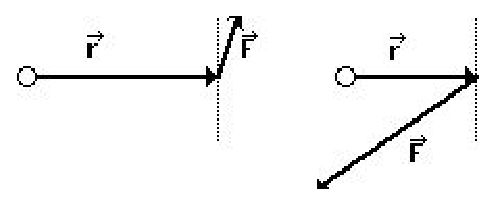
\includegraphics{ang_mom/ang_mom_fig5.eps} \par}
\vspace{0.3cm}

$r =$ \rule{0.5in}{0.1pt} m \hfill{}$F =$ 
\rule{0.5in}{0.1pt} N \hfill{}\( \theta  =\)
 \rule{0.5in}{0.1pt} \hfill{}\( \tau  =\)  \rule{0.5in}{0.1pt} N\( \cdot  \)m 
\vspace{5mm}

$r = $\rule{0.5in}{0.1pt} m \hfill{}$F =$ \rule{0.5in}{0.1pt} N \hfill{}
\( \theta = \)
\rule{0.5in}{0.1pt} \hfill{}\( \tau  =\)  \rule{0.5in}{0.1pt} N\( \cdot  \)m
\vspace{5mm}

\textbf{Momentum and its Rotational Analog} 

Once we have defined the properties of the vector cross product, another important
rotational vector is easily obtained, that of angular momentum relative to an
axis of rotation. 

\textbf{Activity  \stepcounter{activity}\arabic{activity}: Angular and Linear Momentum }

(a) Write the rotational analogs of the linear quantities shown. Note: Include
the formal definition (which is different from the analog) in spaces marked
with an asterisk ({*}). For example the rotational analog for velocity is angular velocity \( \bmath{\omega}  \) and the definition of its magnitude is \( |
\bmath{\omega}  |
= d \theta  /dt\) rather than $v/r$.

\vspace{0.3cm}
{\centering \begin{tabular}{|p{5cm}|p{5cm}|p{5cm}|}
\hline 
Linear Quantity&
Rotational Quantity&
Definition\\
\hline 
\hline 
&
&
\\
$x$ (position) &
&
\\
\hline 
&
&
{*}\\
$v$ (velocity) &
&
\\
\hline 
&
&
{*}\\
$a$ (acceleration) &
&
\\
\hline 
&
&
{*}\\
$F$ (Force) &
&
\\
\hline 
&
&
{*}\\
$m$ (mass) &
&
\\
\hline 
&
&
\\
$F = ma$&
&
\\
\hline 
\end{tabular}\par}
\vspace{0.3cm}

(b) What do you think will be the rotational definition of angular momentum
in terms of the vectors \( {\bf r} \) and \( {\bf p} \)?
\textbf{Hint:} This is similar mathematically to the definition of torque and
also involves a vector cross product. (Note that the symbol for angular momentum is \textbf{L}).
\vspace{20mm}

(c) What is the rotational analog in terms of the quantities $I$ and \( 
\bmath{\omega}  \)? (This is analogous to \textbf{p} = m\textbf{v}.)
Do you expect the angular momentum to be a vector? Explain.
\vspace{30mm}

\textbf{Torque and Change of Angular Momentum }

Earlier in this course you applied a very brief force along a line through the
center of mass of a rolling cart. Do you remember how it moved? What happened
when you applied a gentle but steady force along a line through the center of
mass of the cart? Let's do analogous things to a disk that is free to rotate
on a relatively frictionless bearing, with the idea of formulating laws for
rotational motion that are analogous to Newton's laws for linear motion. 

Figure out how to use a system like that shown in the figure below to observe
the motion of the disk under the influence of a brief torque and a steady torque.
In describing the Laws of Rotational Motion be sure to consider vector properties
and take both the magnitudes and directions of the relevant quantities into
account in your wordings. 

\vspace{0.3cm}
{\par\centering 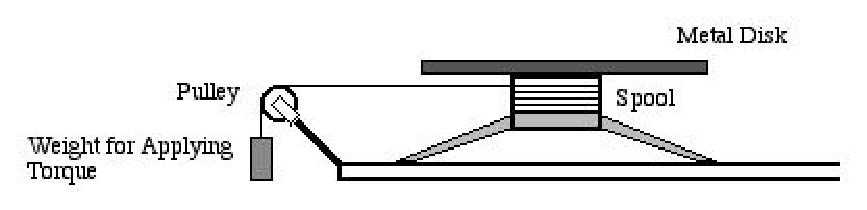
\includegraphics{ang_mom/ang_mom_fig6.eps} \par}
\vspace{0.3cm}

\textbf{Activity  \stepcounter{activity}\arabic{activity}: Applied Torques and Resultant Motion }

(a) After applying a brief torque and then removing the torque, what happens to the angular velocity and hence the angular momentum of the
disk? State a First Law of Rotational Motion in terms of torques and angular momenta. \textbf{Hint:} Newton's first law in translational form states that the center of mass of a system of particles or a rigid object that experiences no net external force will experience no change in linear momentum and so will continue to move at constant velocity.

Newton's First Law in rotational form (in words):
\vspace{20mm}

Newton's First law in rotational form as a mathematical expression: 
\vspace{20mm}

(b) What happens to the magnitude and direction of the angular velocity (and
hence the angular momentum) of the disk during the application of a steady torque? How do they change relative to the magnitude and direction of the torque? If
possible, give a precise statement of a Second Law of Rotational Motion relating the net torque on an object to its change in angular momentum. \textbf{Note:}
Take both magnitudes and directions of the relevant vectors into account in
your statement. \textbf{Hint}: Newton's second law of motion in translational form states that if the center of mass
of a system of particles or rigid object experiences a net external force, it 
will undergo a change in linear momentum such that the rate of change of linear momentum is equal to the net force.

Newton's Second Law of Rotational Motion (in words):
\vspace{20mm}

Newton's Second Law of Rotational Motion as a Vector Equation:
\vspace{20mm}

\textbf{Angular Momentum Conservation }

Now use the vector expression for Newton's Second Law of Rotational
Motion to show that, in theory, we expect angular momentum on a system to be
conserved if the net torque on that system is zero.



\setcounter{activity}{0}

\section{Conservation of Angular Momentum}

Name \rule{2.0in}{0.1pt}\hfill{}Section \rule{1.0in}{0.1pt}\hfill{}Date \rule{1.0in}{0.1pt}

\textbf{Objectives} 

To test the Law of Conservation of Angular Momentum and to explore the applicability
of angular momentum conservation among objects that experience no external torques. 

\textbf{Apparatus}

\begin{itemize}
\item A Rotating Disk System 
\item A mass of 1 kg 
\item A meter stick and a ruler 
\item A small water bubble level
\item A video analysis system
\end{itemize}
\textbf{Overview }

As a consequence of Newton's laws, angular momentum like linear momentum is
believed to be conserved in isolated systems. This means that, no matter how
many internal interactions occur, the total angular momentum of any system should remain constant if there are no external torques. When one of the objects gains some angular momentum another part of the system must lose the same amount. If angular momentum isn't conserved, then we believe that there is some outside torque acting on the system. By expanding the boundary of the system to include the source of that torque we can always preserve the Law of Angular Momentum Conservation. 

In this unit you will test the notion of the conservation of angular momentum.
As in the test of the conservation of linear momentum, we will investigate what
happens when two bodies undergo a ``rotational'' collision.
You will drop a large weight onto a rotating disk and determine the moment of
inertia, the angular speed, and finally, the angular momentum of the rotator-disk-weight
system before and after this perfectly inelastic collision.

\textbf{Activity  \stepcounter{activity}\arabic{activity}: The Moment of Inertia Before and After the Collision}

(a) Calculate the theoretical value of the moment of inertia of the metal disk
using basic measurements of its radius and mass. Be sure to state units and
show the expression you used!
\vspace{5mm}

\( r_{d} =\)  \hfill{}\( M_{d}= \) \hfill{}
\vspace{5mm}

\( I_{d}= \)
\vspace{5mm}

(b) The rotating fixture that holds the disk has a complex shape. We have determined its moment of inertia without the disk and recorded the result. Record that value here. Be sure to state units.
\vspace{5mm}

\( I_{f} =\)
\vspace{5mm}

(c) After dropping the weight on the rotating disk, the system will have a new
moment of inertia. Derive a formula for the moment of inertia of a cylindrical-shaped weight of mass \( m_{w} \) and radius \( r_{w} \) revolving about the origin at a distance \( r_{r} \). (You will have to use the parallel axis theorem to do this.)
\vspace{5mm}

\( I_{w} =\)  
\vspace{5mm}

(d) Measure the mass of the weight and use a vernier caliper to measure its diameter.
\vspace{5mm}

\( m_{w} =\)  \hfill{}\(r_{w} =\) \hfill{}
\vspace{5mm}

(e) Come up with a formula for the moment of inertia $I$ of the whole system
before and after the collision and calculate the moment of inertia before the
collision only. (The moment of inertia after the collision will be determined AFTER you do the experiment, because you will not know \( r_{r} \) until after you do the experiment.) Don't forget to include the units in \( I_{before} \).
\vspace{5mm}

\( I_{\mbox{\small before}}= \) 
\vspace{5mm}

\( I_{\mbox{\small after}} =\)  
\vspace{5mm}

\textbf{Activity  \stepcounter{activity}\arabic{activity}: Making a Movie of the Collision} 

(a) Place the video camera about 1 m above the rotator, align the camera with
the center of the rotator using the pendulum, and center the rotator in the
field of view of the camera by viewing it with the video capture software.
Place a ruler of known length in the field of view of the camera and parallel
to one side of the frame. Check that the rotator is flat with the small water-bubble level.

(b) Give the rotator a push and begin recording its motion with the video camera. 
See \textbf{Appendix D: Video Analysis} for details on making the movie. While the rotator is moving
hold the 1-kg weight near the rim of the metal disk and close to, but not quite
touching, the surface of the moving metal disk. After at least one revolution
of the metal disk drop the 1-kg mass onto the disk and record the motion of
the disk for at least one revolution afterward. 

(c) \textit{Before removing the 1 kg weight from the metal disk}, 
determine the distance of the center of the weight you dropped from the center of the rotator \( r_{r} \). 
To do this, measure the distance from the center
of the rotator to the edge of the weight \( r_{edge} \) and use the result from Activity 1 part (d) 
for the radius of the weight \( r_{w} \). 
Calculate the distance from the origin to the center of the weight \( r_{r} \) (it is just the 
sum of \( r_{edge} \) and \( r_{w} \)). 
Use these results and those from Activity 1 part (e) to calculate the final moment of inertia.
\vspace{5mm}

\( r_{\mbox{\small edge}}  =\) \hfill{}\( r_{w} \) = \hfill{}\( r_{r} \) =\hfill{}
\vspace{5mm}

\( I_{\mbox{\small after}} =\)  
\vspace{5mm}

\textbf{Activity  \stepcounter{activity}\arabic{activity}: Measurement of Angular Velocity}

Determine the angular speed before and after the collision.

(a) Determine the angular displacement of the rotator as a function of time before the weight was dropped. 
To do this task follow the instructions in \textbf{Appendix D: Video Analysis} for recording, calibrating, and analyzing a movie data file. 
\textbf{Important:} Be careful to place the origin of your coordinate system on the axle of the
rotator so the angular displacement you measure will be the desired one. 
Use a marker at or near the edge of the disk to record position for each frame. 
The resulting file should contain three columns with the values of time, $x$-position, and $y$-position.
Calculate the angular position for each time using the $x-$ and $y-$position data, fit the results,
and extract the angular speed of the rotator before the `collision'.

\( \omega _{\mbox{\small before}}=\)

\vspace{5mm}

\newpage

(b) Now follow a similar procedure to determine the angular speed after the collision.
Fit the data and extract the angular speed of the rotator after the `collision'.

\( \omega _{\mbox{\small after}}=\)

\vspace{20mm}

\textbf{Activity  \stepcounter{activity}\arabic{activity}: Calculation of Angular Momentum}

(a) Calculate the angular momentum before and after the collision, including UNITS. Calculate the difference between the two results and record it below. 
Go around to the other lab groups and get their results for the difference between the angular momenta before and after the collision.
Make a histogram of the results you collect and calculate the average and standard deviation.
For information on making histograms, see \textbf{Appendix C}. For information on calculating the average and
standard deviation, see \textbf{Appendix A}. Record the average and standard deviation here.
Attach the histogram to this unit.
\vspace{5mm}

\( L_{\mbox{\small before}}= \)  
\vspace{5mm}

\( L_{\mbox{\small after}}= \)
\vspace{5mm}

\( \Delta L= L_{\mbox{\small after}} - L_{\mbox{\small before}} = \)  
\vspace{30mm}

(b) What is your expectation for the difference between the initial and final angular momentum?
Do the data from the class support this expectation? 
Use the average and standard deviation for the class to quantitatively answer this question.
\vspace{20mm}


(c) Within the limits of experimental uncertainty, is angular momentum 
conserved?  Be quantitative.
\vspace{20mm}

(c) Would the procedure you followed above change if the weight was moving horizontally at a constant velocity when you dropped it? 
If it changed, what would be different?
\vspace{20mm}




% appendices.

P7 332
#XVVERSION:version 3.10a-jumboFix+Enh of 20081216 (interim!)+FLmask
#BUILTIN:UNKNOWN
#IMGINFO:
#END_OF_COMMENTS


P7 332
#XVVERSION:version 3.10a-jumboFix+Enh of 20081216 (interim!)+FLmask
#BUILTIN:UNKNOWN
#IMGINFO:
#END_OF_COMMENTS


P7 332
#XVVERSION:version 3.10a-jumboFix+Enh of 20081216 (interim!)+FLmask
#BUILTIN:UNKNOWN
#IMGINFO:
#END_OF_COMMENTS



\section{Video Analysis}

\textbf{Making a Movie with ``Windows Live Movie Maker''} 

To make a movie, perform the following steps:

\begin{enumerate}

\item Make sure the camera is connected to a USB port on your computer. 
Close all windows, applications, programs, and browsers.

\item Click the {\bf Start} button in the lower-left corner of your screen and type `movie maker' in the Search programs and files box. 
Once the search results appear, click on {\bf Windows Live Movie Maker} under {\bf Programs}. 
After movie maker starts, close any pop-up windows that may appear.

\item Click the {\bf Webcam Video} button. 
A webcam video window opens. 
Enlarge the video frame by dragging the vertical line on the right side of the video frame.

\item Position the camera 2-3 meters from the object you will be viewing. 
Adjust the camera height and orientation so that the field of view is 
centered on the expected region where the object will move. 

\item Place a meter stick or an object of known size in the field of view where 
it won't interfere with the experiment. 
The meter stick should be the same distance away from the camera as the motion 
you are analyzing so the horizontal and vertical scales will be accurately determined. 
It should also be parallel to one of the sides of the movie frame. 
Make sure that the meter stick is not far away from the central region of field of view, and that it is perpendicular to the line of sight of camera.

\item One member of your group should perform the computer tasks while the other does the experiment.

\item To start recording your video, click {\bf Record}. When you are done, click {\bf Stop}. 

Save the video on your Desktop with a unique name that you can easily identify.
 The video will be saved in Windows Media Video format, i.e. with extension wmv. (Do not save the video as a Movie Maker Project file.)

\end{enumerate}

\textbf{Analyzing the Movie} 

To determine the position of an object at different times during the
motion, perform the following steps:

\begin{enumerate}

\item Start up Tracker by going to {\bf Start} $\rightarrow$ {\bf All Programs} $\rightarrow$ 
{\bf Physics Applications} $\rightarrow$ {\bf Tracker}. 
When {\bf Tracker} starts it appears as shown below. The menu icons and buttons that we will use are identified by arrows.
\begin{figure}[hbt]
\begin{center}
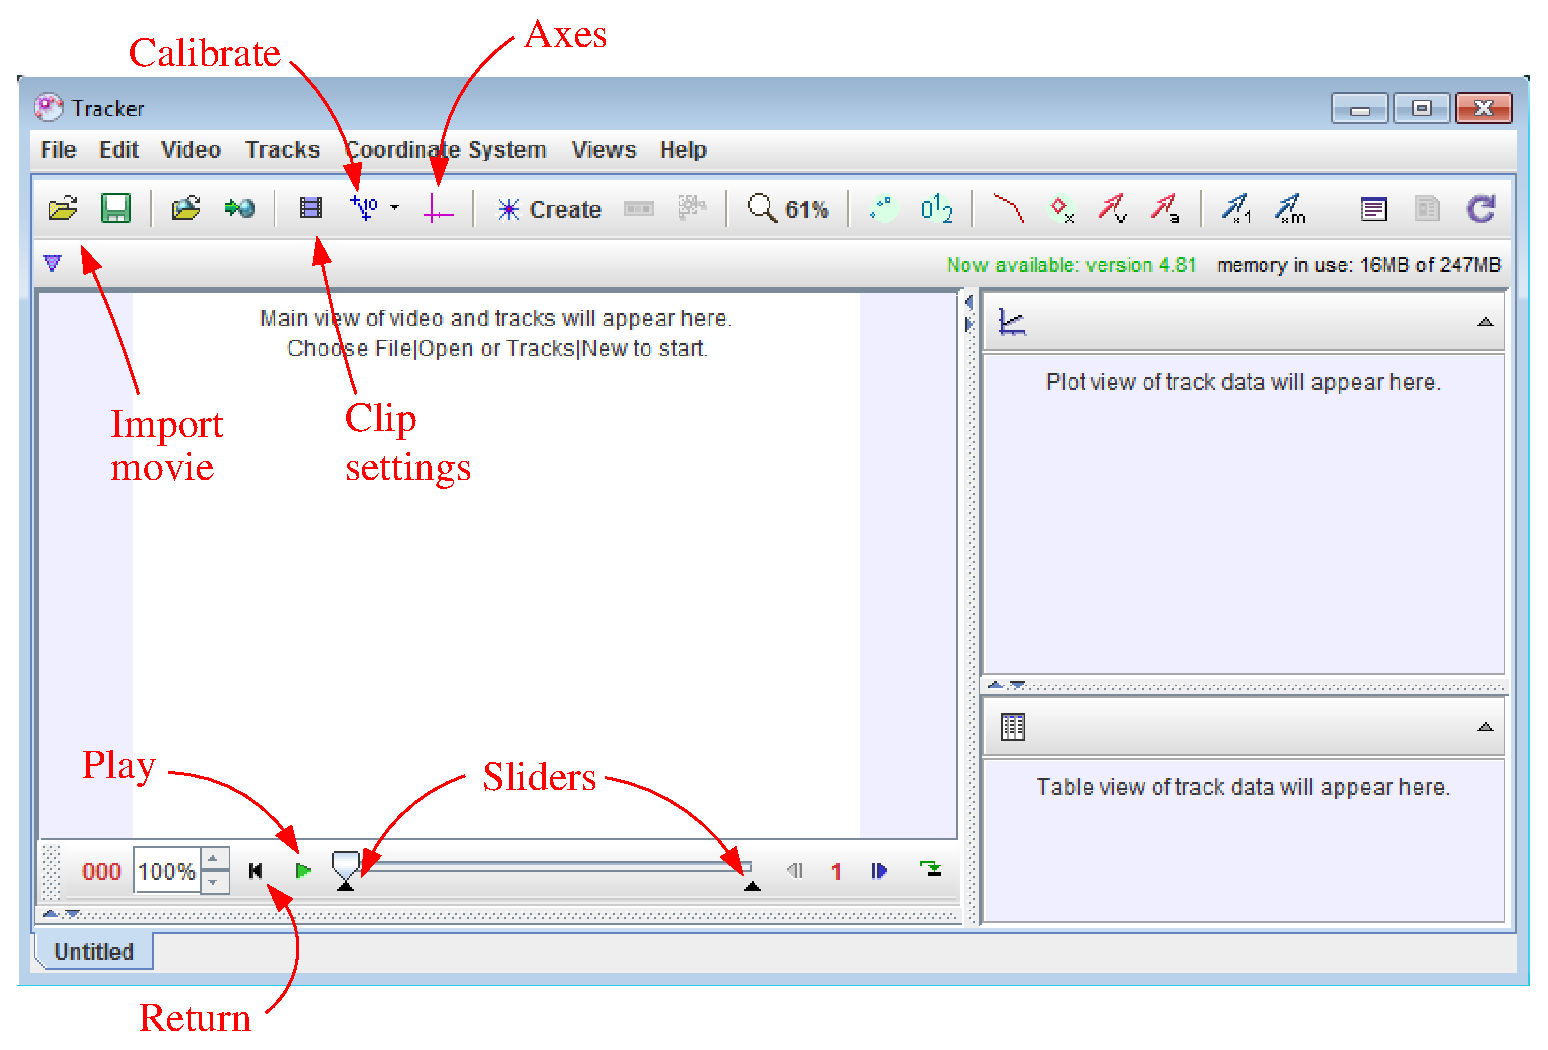
\includegraphics[width=5.5in]{appendices/video_analysis_tracker_fig1d.eps}
\caption{Initial {\bf Tracker} window for video analysis.}
\end{center}
\end{figure}

\item Click the {\bf Open Video} button on the toolbar (see figure below) to import your video. 
After your video is imported, Tracker will warn you that the video frames don't have the same time duration. 
This is okay since Windows Live Movie Maker uses a variable frame rate. 
Click {\bf Close} on the warning window to ignore Tracker's recommendation.

\item Click the {\bf Clip Settings} button (see figure below) to identify the frames you wish to analyze. 
A clip settings dialog box appears. 
Here, you only need to identify and set the start and end frames. 
Leave everything else in the dialog box unchanged. 
To find and set the start frame, drag the player's left slider to scan forward through the video, and 
stop when you get to the first frame of interest. 
Now, the start frame is set and the corresponding frame number should be displayed in the dialog box. 
If not, then click on the {\bf Start Frame} in the dialog box, enter the number of the frame 
(printed in the lower right part of the Tracker window), and click outside the box.
Then, click the {\bf Play video} button to go to the last frame in the video. 
Next, drag the player's right slider to scan backward through the video to find the last frame of interest. 
Stop when you get to the frame of interest. Now, the end frame is also set and the corresponding frame number should be displayed in the dialog box. 
If not, then click on the {\bf End Frame} in the dialog box, enter the number of the frame, and click outside the box.
Finally, click the {\bf OK} button to close the dialog box, and then click the player's {\bf Return} button to return to the start frame.

\item Click the {\bf Calibration} button (see the figure) and select the {\bf calibration stick}. 
A blue calibration line appears on the video frame. 
Drag the ends of this blue line to the ends of your calibration meter stick. 
Then click the readout box on the calibration line to select it. 
Enter the length of the meter stick in this box (without units). 
For example, if your calibration meter stick is 1.00 meter long, enter 1.00 in the box 
and then click outside the box to accept the value or hit {\bf Return}. 
At this point, you can right-click the video frame to zoom in for more accurate adjustment of the ends 
of the calibration stick. 
Right-click the video again to zoom out.

\item Click the {\bf Axes} button (see the figure) to set the origin and orientation of the x-y coordinate axes. 
Drag the origin of the axes to the desired position (in most cases the initial position of the object of interest). 
Click the video outside the origin to fix the position of the origin. 
To change the orientation (angle) of the axes, drag the x axis. 
Click the video to fix the new orientation.

\item Click the {\bf Create} button (see the figure) to track the object of interest in the video. 
From the menu of choices select {\bf Point Mass} for the track type. 
Make sure the video is at the start frame, which shows the initial position of the object of interest. 
Mark this position by holding down the {\bf shift key} and clicking the mouse (crosshair cursor) on the object. 
As the position is marked, the video automatically advances to the next frame. 
Similarly, mark the position of the object on this and subsequent frames by holding down the {\bf shift key} 
and clicking the mouse. 
Do not skip any frames. 

After marking the position on the end frame, you can adjust any one of the marked positions. 
Advance the video to the frame where you would like to make a fine adjustment. 
Right-click the video frame to zoom in and drag the marked position with the mouse.

If you would like to track additional objects, repeat the procedure outlined here for each object.

\item Click the {\bf Set track length} button (see the figure) to get a drop-down menu that
will enable you to show all of the points you marked on the frame.

\item {\bf Plotting and Analyzing the Tracks:} The track data (position versus time) are listed in the Table View 
and plotted in Plot View sections of the Tracker screen. 
Click the vertical axis label of the plot to change the variable plotted along that axis. 
To plot multiple graphs, click the {\bf Plot} button, located above the plot, and select the desired number. 

Right-click on a plot to access display and analysis options in a pop-up menu. 
To fit your data to a line, parabola, or other functions, select the {\bf Analyze} option. 
On the Data-Tool window that opens up, click on the {\bf Analyze} tab at the top of the plot and 
check the {\bf Curve Fits} box. Select the fit type from the {\bf Fit Name} drop-down menu.
Make sure the {\bf Auto Fit} box is checked.


Note that the curve fitter fits the selected function to the data in the two leftmost columns of the displayed data table. 
The leftmost column, identified by a yellow header cell, defines the independent variable, and the second leftmost column, 
identified by a green header cell, defines the dependent variable. 
So, to fit the data in other columns, their corresponding headers must be dragged to the two leftmost columns.


\item {\bf Printing and Exporting Data:} Track data can also be easily exported to Excel for 
further analysis by copying the data from the 
data table to the clipboard and pasting into Excel. 
Click the {\bf Table} button, located above the data table in the table view section of the main screen, 
and select from the displayed list the data you would like to display in the data table. 
Select the desired data in the table by clicking and dragging, then right-click and choose {\bf Copy Data} 
from the pop-up menu. 
Now, paste the data into Excel.
To print out the displayed  plot or data table on Tracker's screen, 
right-click on the plot or table and choose Print from the pop-up menu.

\end{enumerate}



P7 332
#XVVERSION:version 3.10a-jumboFix+Enh of 20081216 (interim!)+FLmask
#BUILTIN:UNKNOWN
#IMGINFO:
#END_OF_COMMENTS


\end{document}
